\documentclass[aspectratio=169,10pt]{beamer}
\usetheme{default}
\usecolortheme{seahorse}
\setbeamertemplate{navigation symbols}{}
\setbeamertemplate{footline}[frame number]
\usepackage{graphicx, booktabs, siunitx}
\graphicspath{{../figures/run224460/}{../figures/}}
\title{Run 224460 Follow-up: Arms A/D Recovered,\\ SiPM-Wall Channel Autopsy}
\subtitle{n\_TOF EAR2 X17 --- run 224460 (July 16, after plastic operating-point change)}
\author{Dylan Neff \\[0.5ex] {\small analysis and slides prepared with Claude (Anthropic AI assistant)}}
\date{July 17, 2026}

\begin{document}

\begin{frame}\titlepage\end{frame}

\begin{frame}{Data \& selection}
\begin{itemize}
\item Official processed file, run 224460: 4005 bunches (2058 dedicated),
      $\sim$335M WAL/PSS hits ($\sim$25\% more than 224404).
\item \textbf{No SiPM-wall outage this run} --- all 3943 beam-on bunches used
      (224404 lost 46\%).
\item \alert{The official \texttt{index} tree is empty in this run} --- pipeline now
      falls back to \texttt{PKUP} (one entry/bunch, identical intensities); the
      224404 bunch mask is applied per run.
\item Between the runs the \textbf{plastic PMT operating points changed}: every PSS
      channel's spectral structure moved up $\sim\!2\times$; PSSA thresholds
      deepened ($-14/-13 \to -19/-18$ mV). Walls unchanged.
\item Selection as before: beam-on bunches, hits $>$0.1 ms after $\gamma$-flash.
\end{itemize}
\end{frame}

\begin{frame}{Headline: the A/D coincidence deficit is gone}
\centering
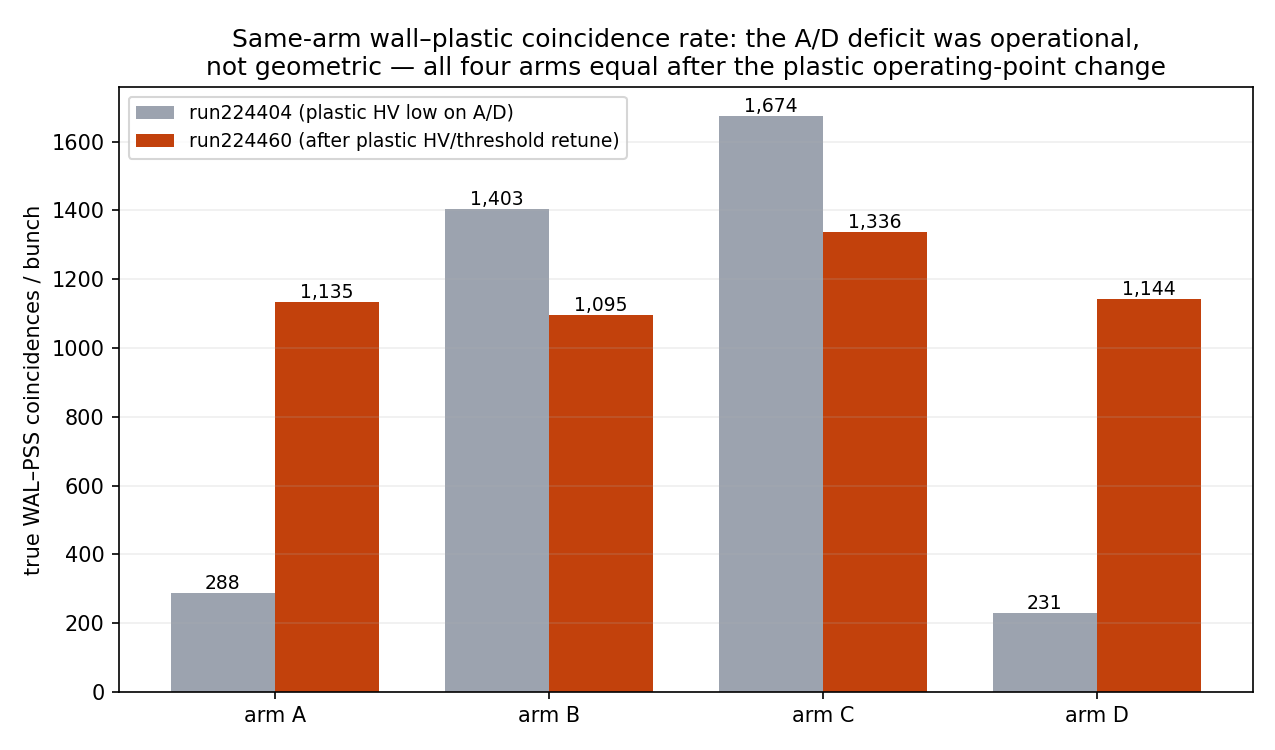
\includegraphics[height=.72\textheight]{arm_rate_comparison.png}\\
{\footnotesize Same-arm true coincidences per bunch. A: $288\to1135$,
D: $231\to1144$ ($4$--$5\times$); B/C stable. All four arms now agree within
$\pm$11\%. \textbf{The 224404 deficit was the plastic operating point ---
not geometry, mapping, or cabling.}}
\end{frame}

\begin{frame}{All 16 wall--plastic pairs, calibrated dt}
\centering

\includegraphics[height=.72\textheight]{02_coincidence/dt_matrix.png}\\
{\footnotesize Diagonal excesses 4.3--5.3M, cross pairs 0.19--0.35M;
$P(\text{wall}\,|\,\text{plastic hit})=12$--$14\%$ on \emph{all} arms
(was 2\% on A/D in 224404).}
\end{frame}

\begin{frame}{Channel mapping re-confirmed with full contrast}
\centering

\includegraphics[height=.68\textheight]{04_channel_mapping/channel_mapping.png}\\
{\footnotesize Bar-1 share falls 0.90$\to$0.10 across channels 1$\to$8 on
\emph{every} arm (A/D were washed out to 0.7/0.3 in 224404 by shower-dominated
samples). Plastic ch1 = left, wall pairs (1,2)$\ldots$(7,8) = groups
left$\to$right seen from the back --- in stone.}
\end{frame}

\begin{frame}{MIP peaks on all 32 SiPM-wall channels}
\centering

\includegraphics[width=\textwidth]{06_07_geometry_mip/mip_wall_spectra_linear.png}\\
{\footnotesize Sideband-subtracted coincidence spectra: two-component shape
(accidentals $\sim$5 mV + MIP) everywhere. B/C/D$_{1\text{--}6}$: 33--43 mV.
\alert{WALA all channels $\sim$30\% low (22--28 mV); WALD ch7/ch8 low and
distorted} $\Rightarrow$ next slides.}
\end{frame}

\begin{frame}{Odd-channel autopsy 1: partner-tagged response (no plastic involved)}
\centering
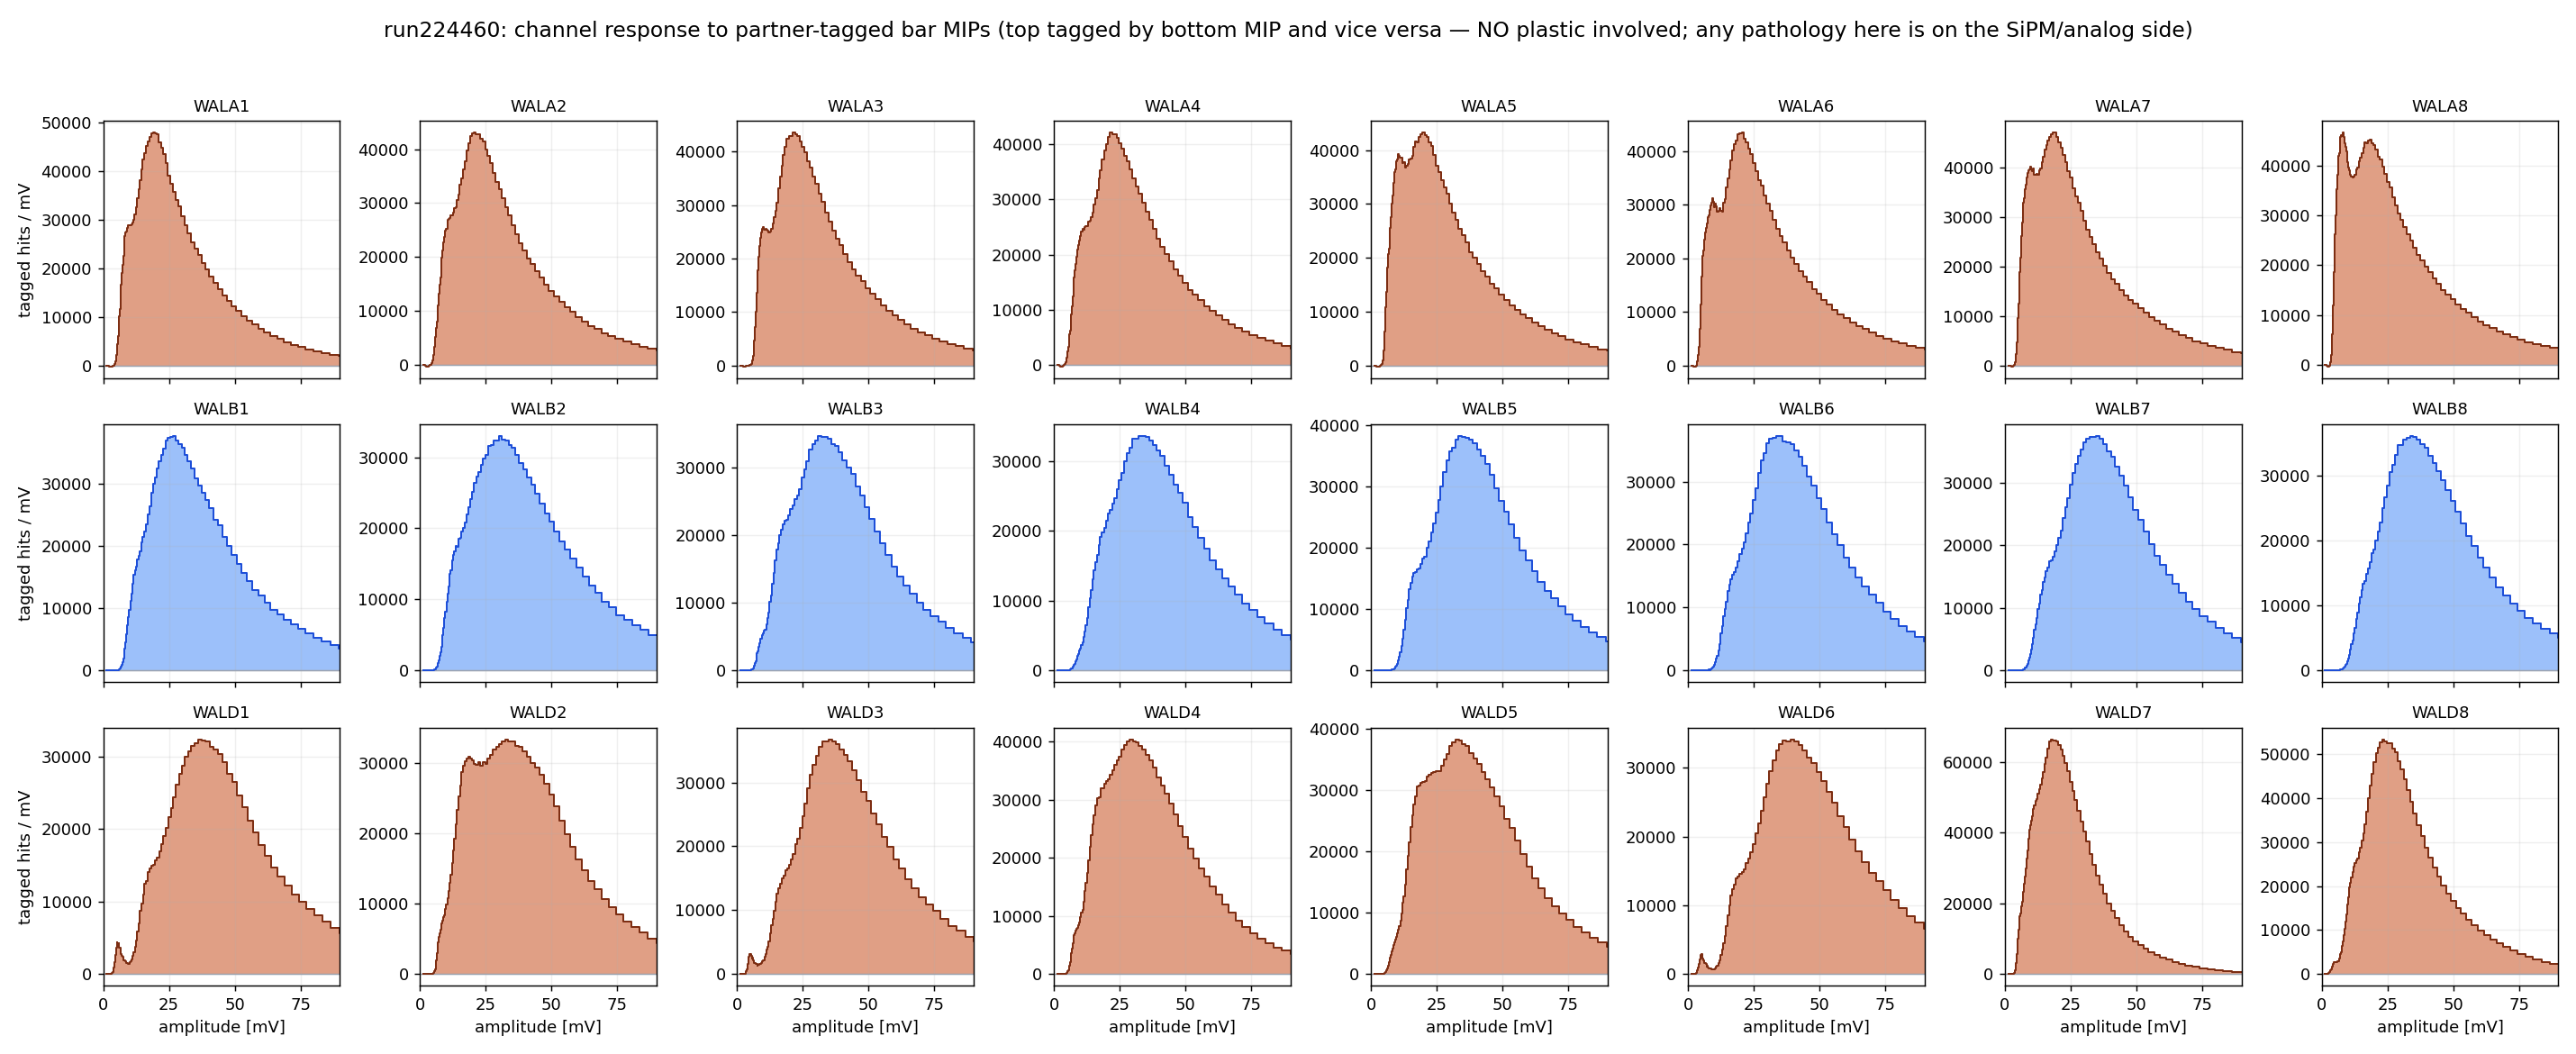
\includegraphics[width=.92\textwidth]{autopsy/tagged_spectra.png}\\
{\footnotesize Each channel's response to bar-MIPs tagged by the \emph{other end}
of the same bars --- plastic plays no role. Every channel shows a Landau, but:
WALA uniformly low (24--29 mV tagged modes vs 35--43 mV on B);
\alert{WALD7 = 23 mV, WALD8 = 29 mV vs 38--48 mV for WALD g1--g3}.
The pathology lives on the \textbf{SiPM/analog side}; the plastics are exonerated.}
\end{frame}

\begin{frame}{Odd-channel autopsy 2: it is signal \emph{duplication}, not cross-talk}
\centering
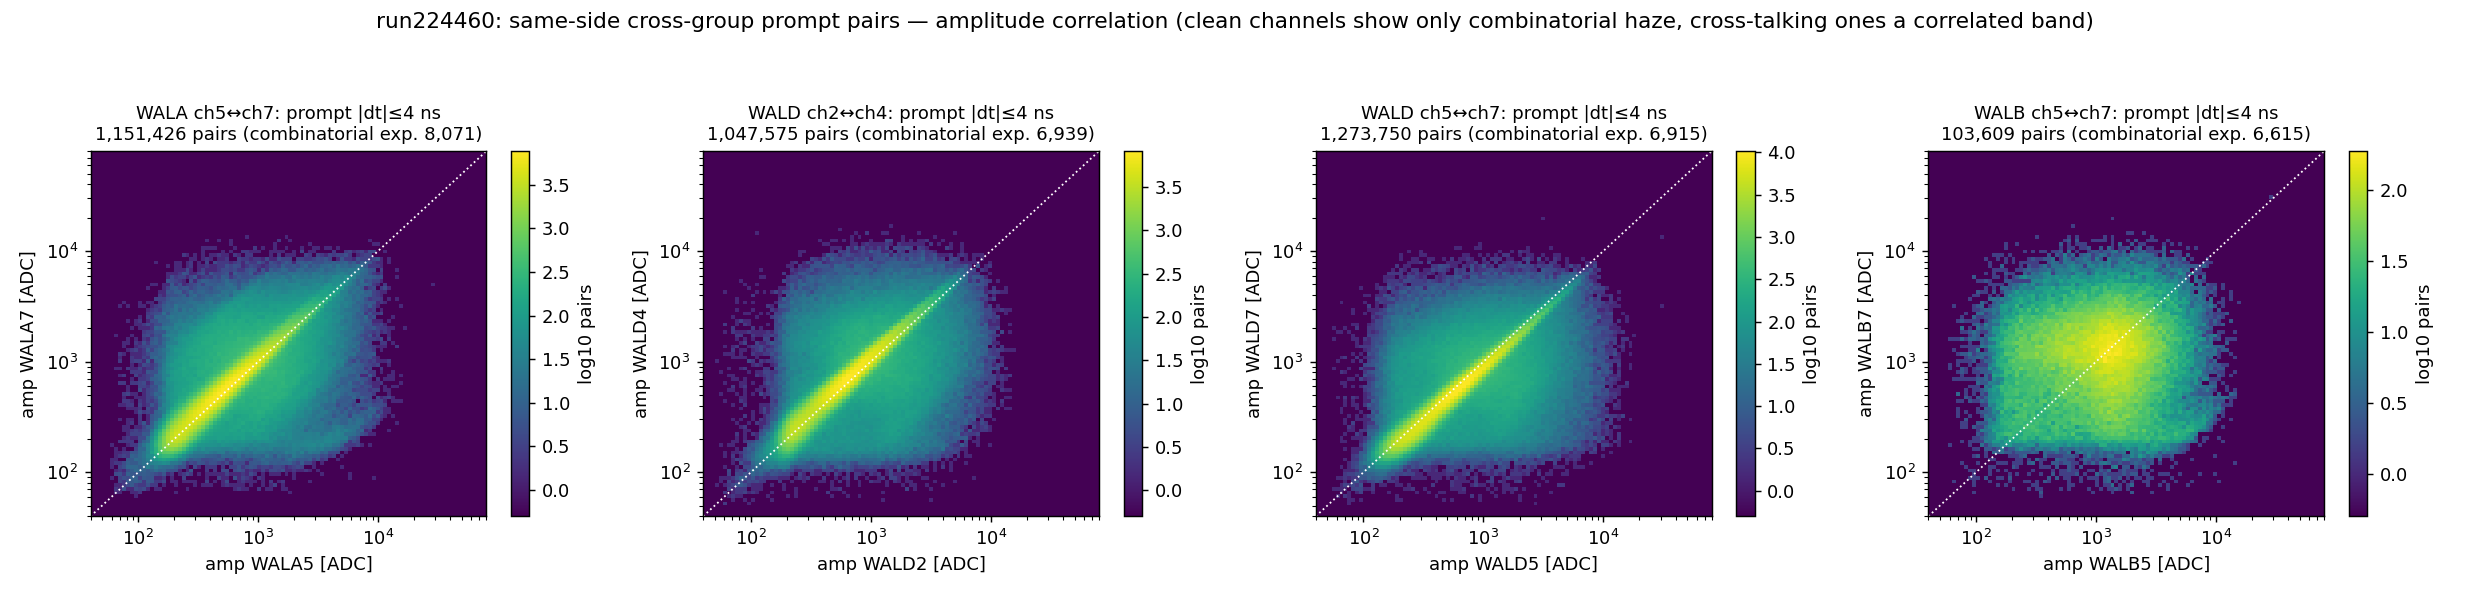
\includegraphics[width=\textwidth]{autopsy/xtalk_2d.png}\\
{\footnotesize Prompt ($|dt|\le4$ ns) same-side cross-group pairs. WALA 5$\leftrightarrow$7,
WALD 2$\leftrightarrow$4, WALD 5$\leftrightarrow$7: 1.0--1.3M pairs on a razor-sharp
\textbf{equal-amplitude diagonal} (combinatorial expectation $\sim$7k; mean ratio
0.8--1.1) --- the \emph{same pulse} appears on both channels. Clean reference (WALB
5$\leftrightarrow$7, right): combinatorial haze only. Capacitive cross-talk would sit
far below the diagonal $\Rightarrow$ look for a shorted/split analog path
(SiPM summing board, patch panel, or splitter) on those channel pairs.}
\end{frame}

\begin{frame}{The duplication explains the deformed spectra --- and a veto cleans them}
\centering
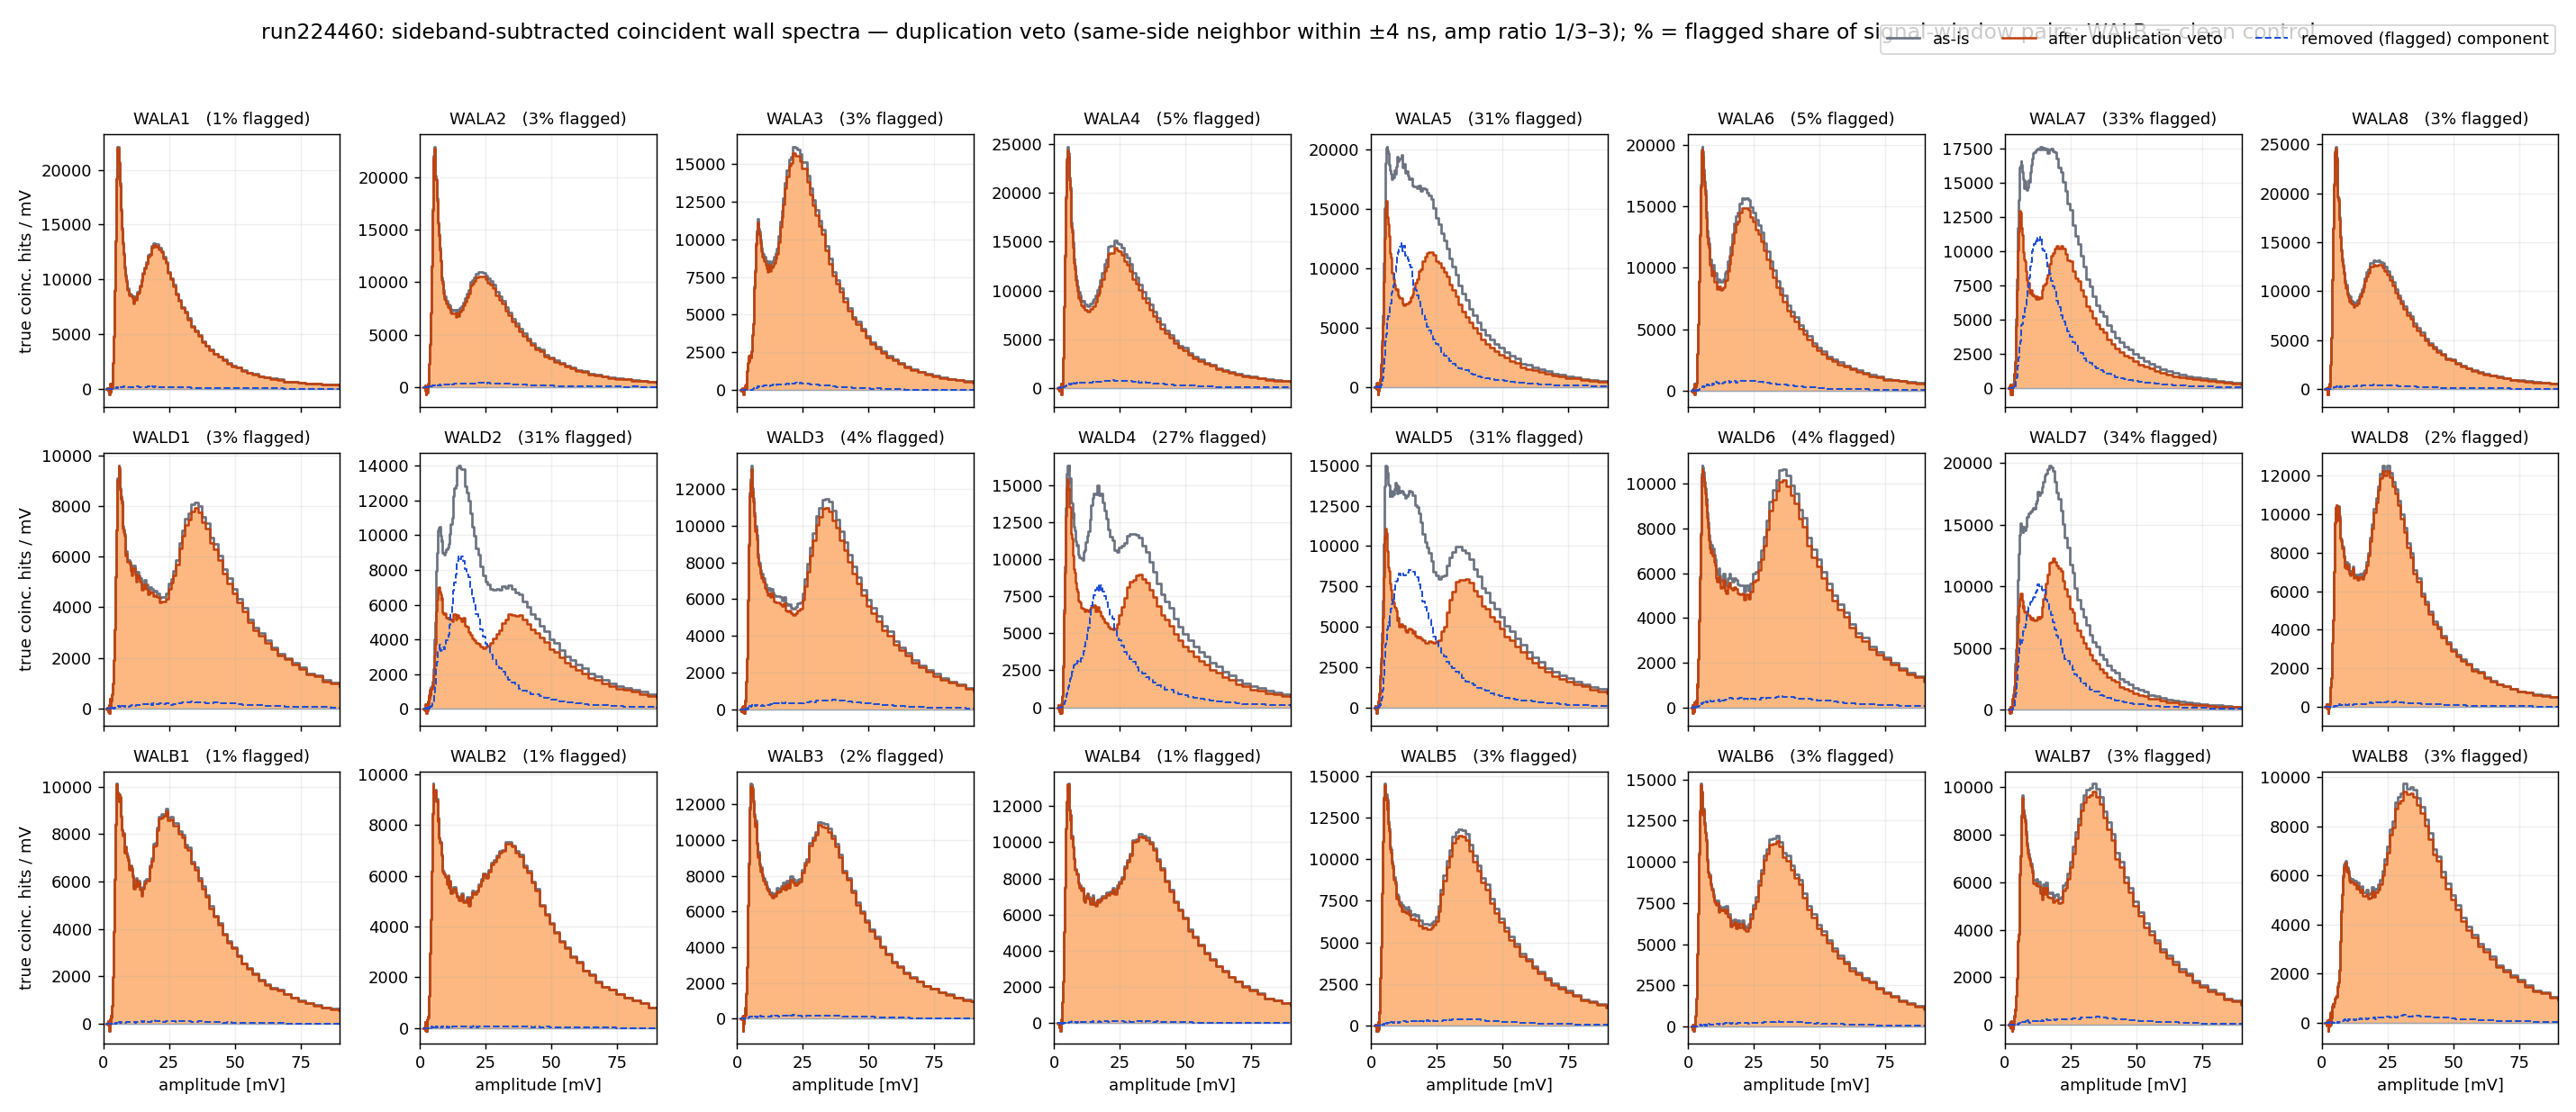
\includegraphics[width=.94\textwidth]{autopsy/dup_veto_spectra.png}\\
{\footnotesize Veto: same-side neighbor hit within $\pm$4 ns with amplitude ratio
1/3--3. Flagged share of signal-window pairs: \textbf{27--34\% on exactly the
duplicated channels}, 1--5\% elsewhere, $\le$3\% on all of WALB (control,
spectra untouched). The removed component (blue dashed) \emph{is} the deformation;
survivors are clean Landaus (e.g.\ WALD7: broad hump $\to$ well-formed MIP at
$\sim$21 mV --- its gain is still genuinely low). Channels keep 62--71\% of their
excess $\Rightarrow$ software cleaning is viable until the analog fix.}
\end{frame}

\begin{frame}{Channel verdicts \& requests}
\small
\begin{columns}[T]
\column{.52\textwidth}
\textbf{Verdicts (all SiPM/analog side):}
\begin{itemize}
\item WALA (all 8): gain $\sim$30\% low; several same-side channel pairs weakly
      correlated --- check wall-A analog section / bias.
\item WALA 5$\leftrightarrow$7, WALD 2$\leftrightarrow$4, WALD 5$\leftrightarrow$7:
      equal-amplitude signal duplication (present and identical in 224404 and
      224460) --- inspect cabling/summing for these pairs.
\item WALD ch7/ch8 (group 4): genuinely weak response (tagged MIP $\sim$40\% low)
      --- bias/SiPM check.
\item Plastics: healthy on all arms at the new operating point; PSSC1 (junk-dominated)
      and PSSD2 (low mode) worth an eye during the HV scan analysis.
\end{itemize}
\column{.44\textwidth}
\textbf{Requests:}
\begin{enumerate}
\item Inspect/swap analog paths of the three duplicated channel pairs before
      the next long run; a bench pulser check pinpoints the split.
\item HV/gain trim: wall A (all), wall D group 4; then re-derive MIP constants.
\item DAQ: why is the \texttt{index} tree empty in 224460?
\item Plastic HV scan analysis (in progress) $\to$ gain equalization; keep the
      224404 operating point documented as the ``do not use'' reference.
\end{enumerate}
\end{columns}
\end{frame}

\begin{frame}{Trigger thresholds: top+bottom sum, one threshold per wall}
\centering

\includegraphics[width=\textwidth]{18_trigger/threshold_scan.png}\\[0.5ex]
\scriptsize
\begin{tabular}{lccccc}
\toprule
wall & \textbf{rec.\ thr} & eff g1--g4 & purity g1--g4 & pairs/bunch & dup.\ unfixed \\
\midrule
WALA & \textbf{12 mV} & .96/.99/.98/.98 & .92--.94 & 2454 & 2878 (+17\%) \\
WALB & \textbf{14 mV} & .97/.96/.96/1.0 & .88--.91 & 2916 & 2981 (+2\%) \\
WALC & \textbf{12 mV} & .96/.96/.97/.98 & .84--.88 & 3184 & 3293 (+3\%) \\
WALD & \textbf{14 mV} & .99/.96/.97/.97 & .85--.94 & 2526 & 3168 (+25\%) \\
\bottomrule
\end{tabular}\\[0.5ex]
{\footnotesize Rule: weakest group of each wall kept at $\ge$95\% MIP efficiency;
thresholds $\approx$20--30\% of the lowest group's MIP-sum peak (WALA low gain,
WALD g4 weak). Duplication cannot be vetoed in hardware $\Rightarrow$ fix the
analog paths before freezing rates. Details: \texttt{TRIGGER\_THRESHOLDS.md}.}
\end{frame}

\begin{frame}{Trigger-candidate top+bottom sum spectra with recommended cut}
\centering
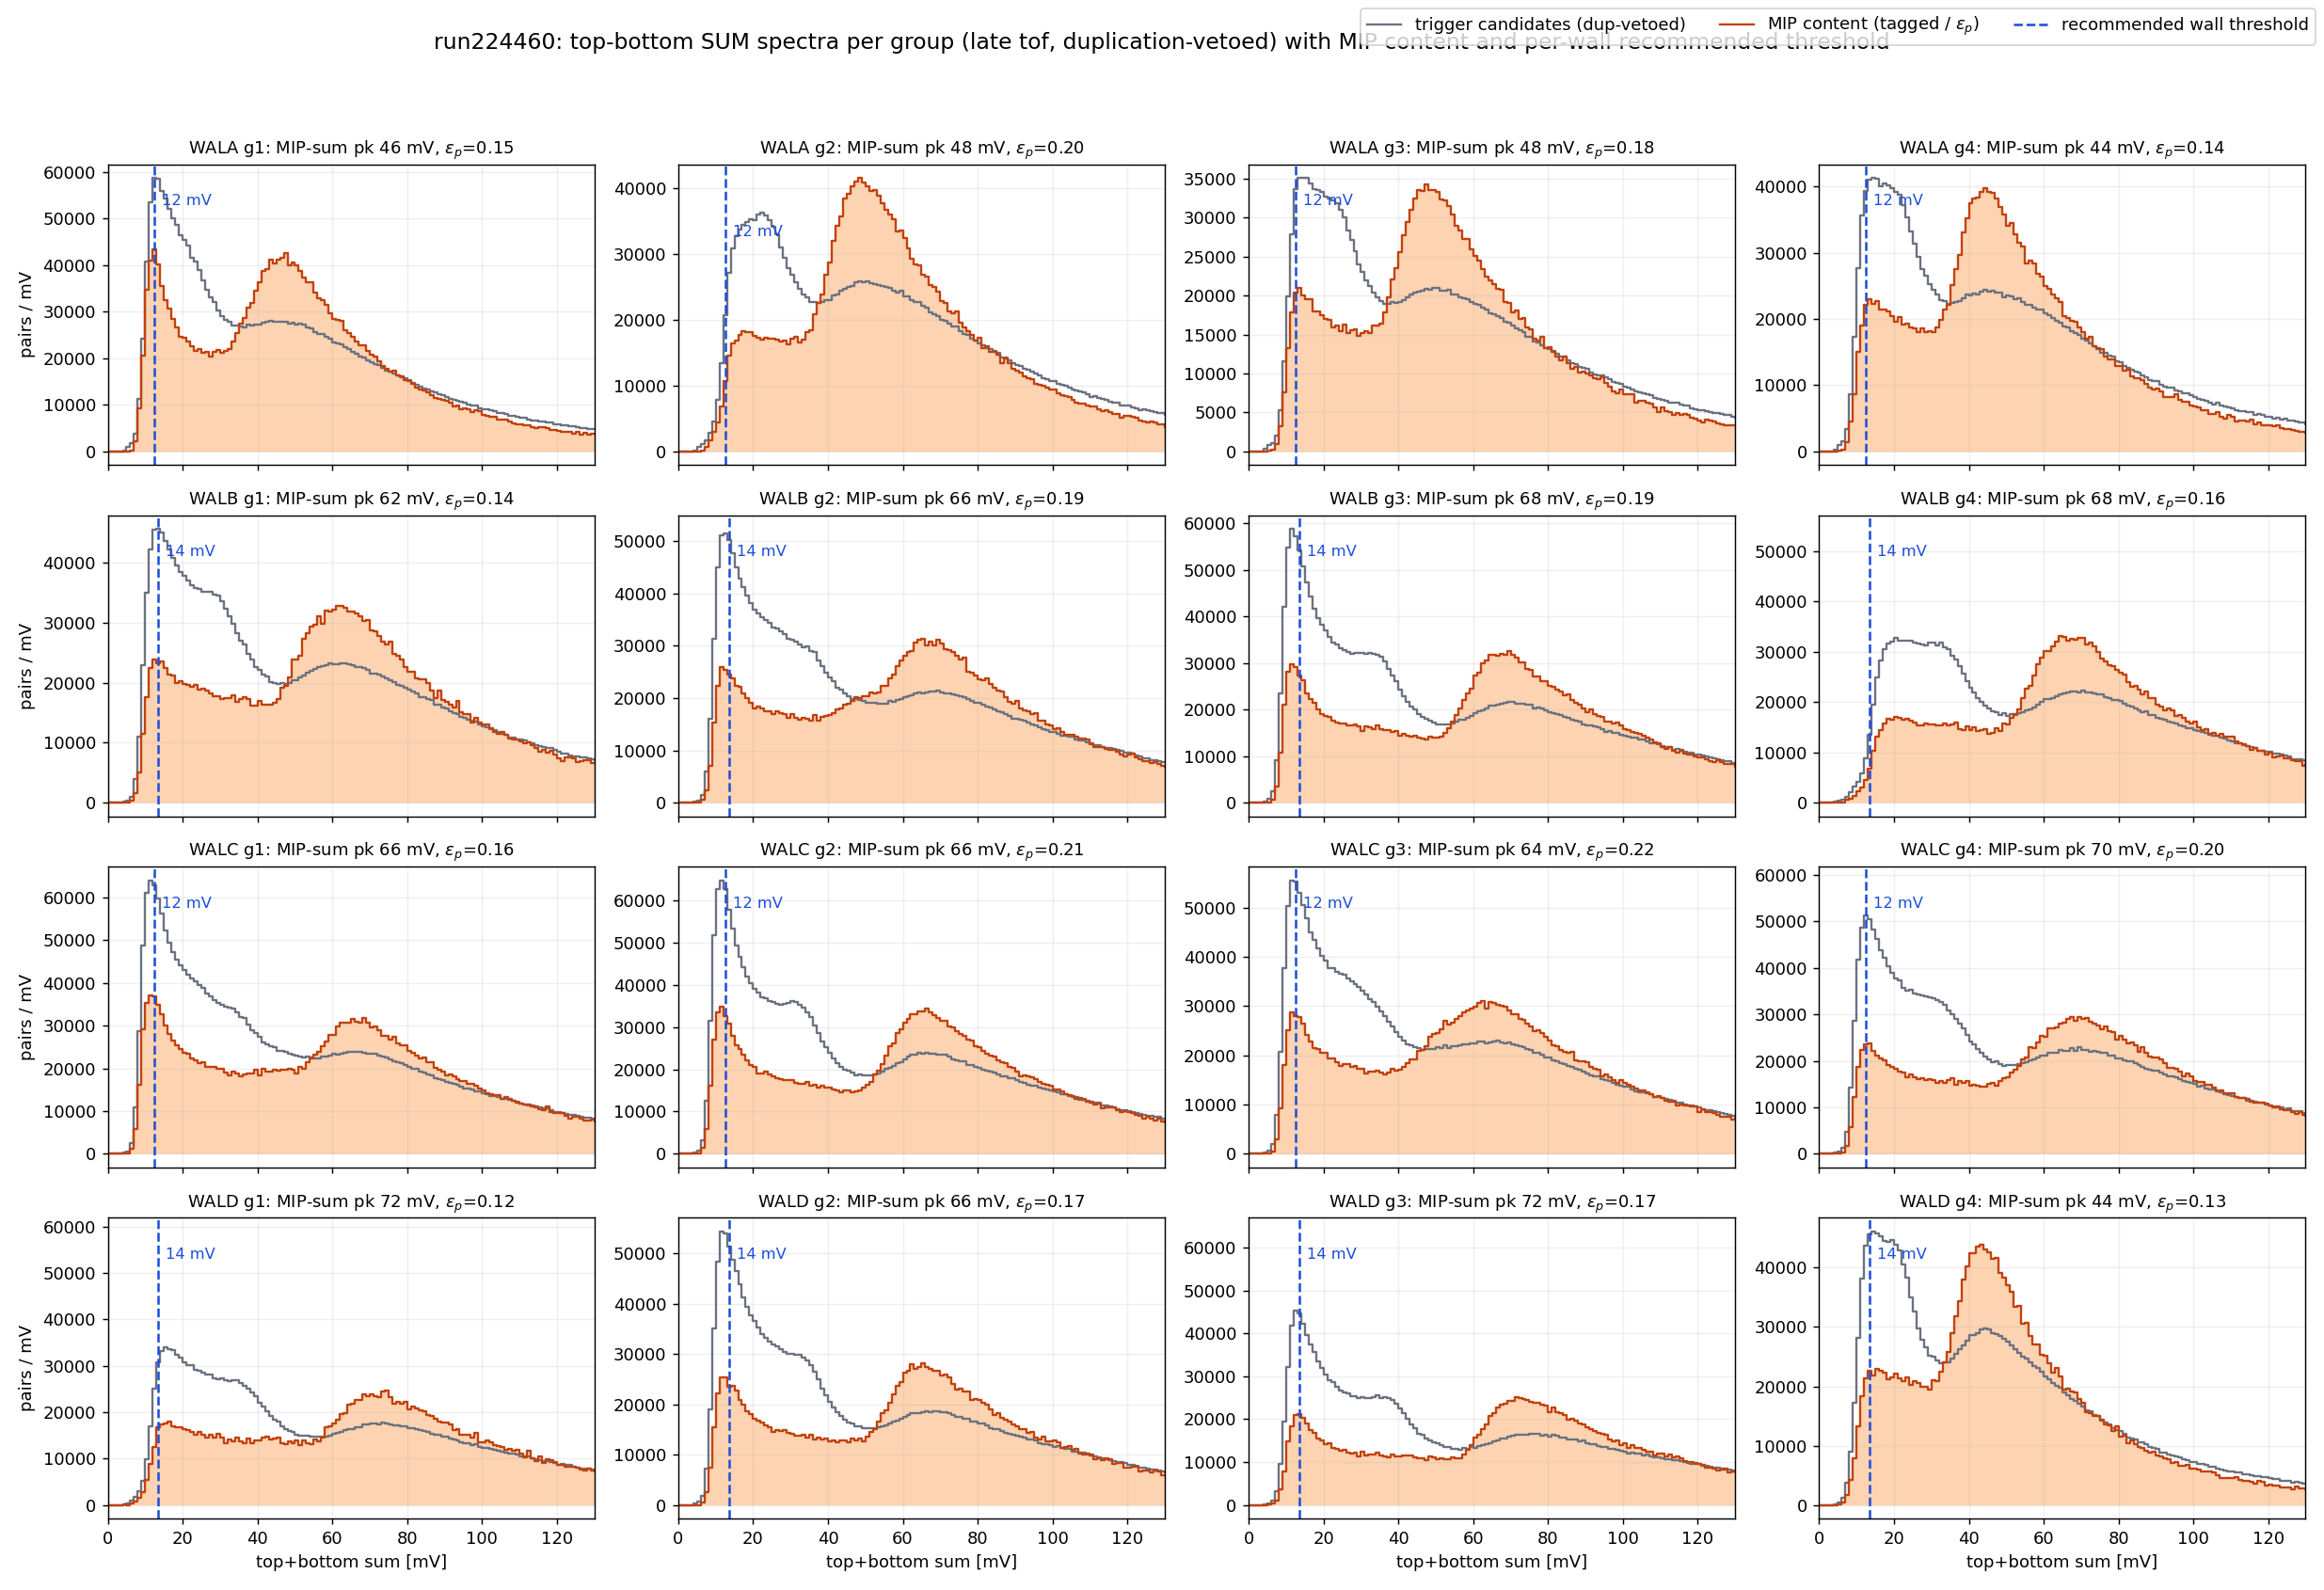
\includegraphics[height=.78\textheight]{18_trigger/trigsum_spectra_linear.png}\\
{\tiny Log-scale variant: \texttt{18\_trigger/trigsum\_spectra.png}. MIP content
$>$ candidates near the bump on some panels: $\epsilon_p$ grows with sum, so
quoted purities at threshold are conservative.}
\end{frame}

\begin{frame}{Backup: purity vs efficiency per group}
\centering
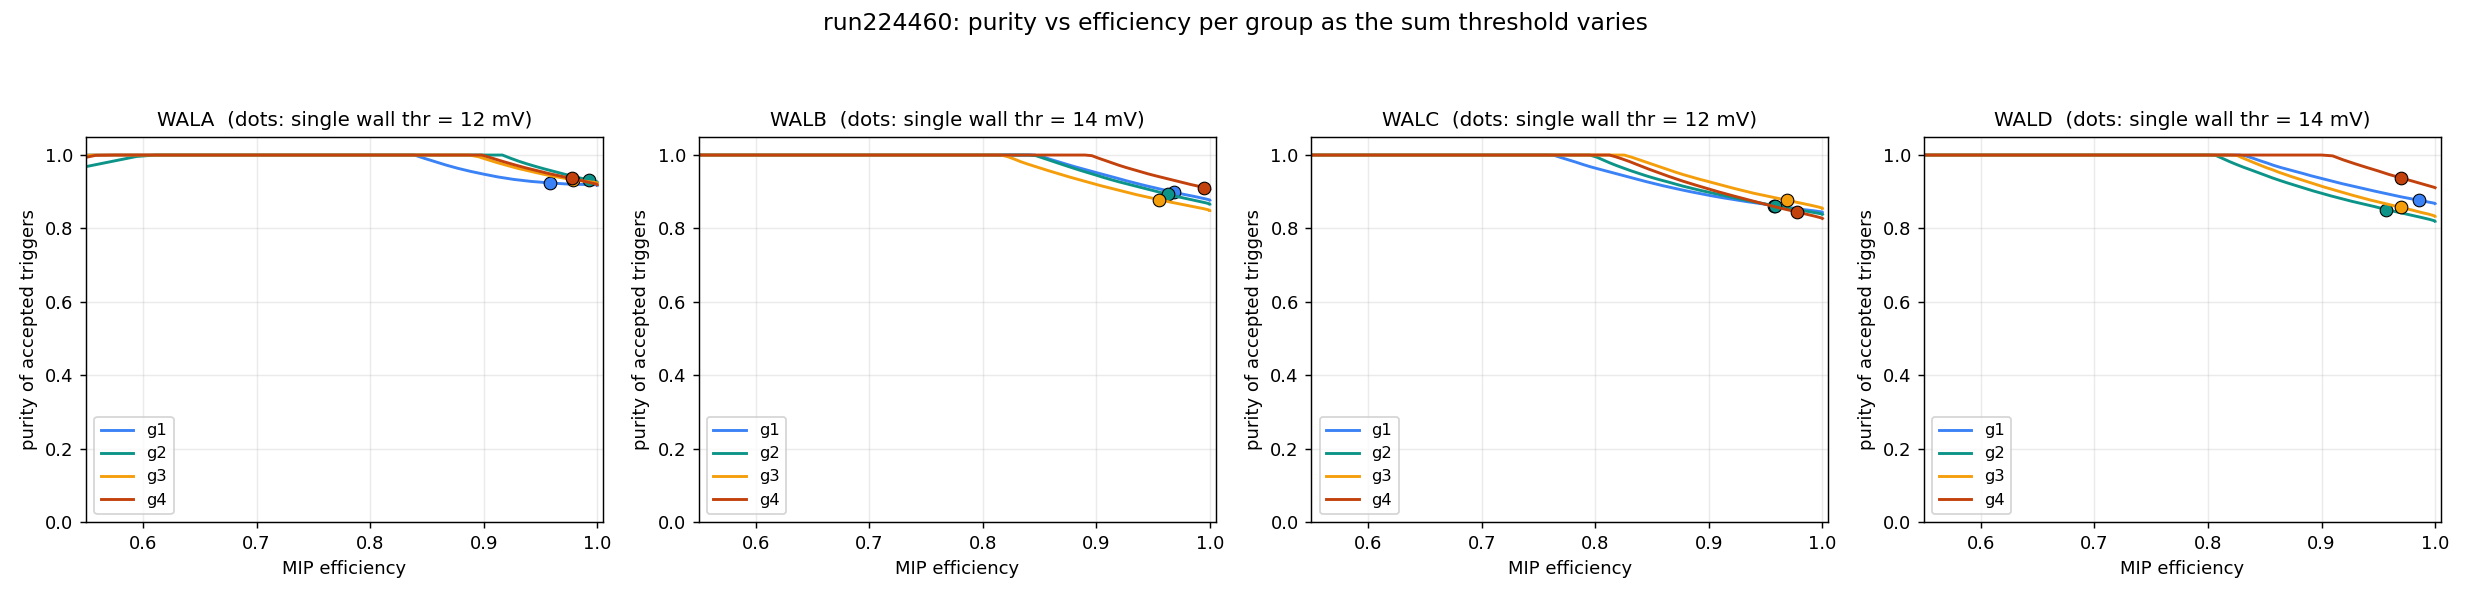
\includegraphics[width=\textwidth]{18_trigger/purity_vs_eff.png}
\end{frame}

\begin{frame}{Backup: dt by time-since-flash region}
\centering

\includegraphics[width=.9\textwidth]{02_coincidence/dt_by_region.png}
\end{frame}

\begin{frame}{Backup: window scan \& purity (arm A, now healthy)}
\centering

\includegraphics[width=.9\textwidth]{02_coincidence/window_scan_regions_WALA_PSSA.png}
\end{frame}

\begin{frame}{Backup: plastic coincident spectra}
\centering

\includegraphics[width=.95\textwidth]{06_07_geometry_mip/mip_pss_spectra.png}
\end{frame}

\begin{frame}{Backup: rate stability over the run}
\centering

\includegraphics[width=.85\textwidth]{01_signal_qa/rate_stability.png}
\end{frame}

\end{document}
